\thm $\zeta(z)$ can be extended to be holomorphic in $\C\setminus\brace1$ with a simple pole of residue $1$ at $1$. \\
\pf
\[ \int_0^\infty t^{z-1} e^{-nt} \d t = \dotsb = \frac1{n^z}\Gamma(z) \]
For $\Re(z)>1$,
\begin{align*}
\zeta(z) &= \sum_{n=1}^\infty\frac1{n^z} = \sum_{n=1}^\infty \frac1{\Gamma(z)}\int_0^\infty t^{z-1}e^{-nt}\d t \\
&= \frac{1}{\Gamma(z)}\int_0^\infty t^{z-1} \frac{e^{-t}}{1-e^{-t}} \d t \\
\zeta(z) &= \frac1{\Gamma(z)}\int_0^\infty t^{z-1}\paren[\Big]{\frac1{e^t-1}}\d t
\end{align*}
for $\Re(z)>1$.

We wish to show that $\zeta(z)-\frac1{z-1}$ is holomorphic in $\C$
\begin{align*}
\zeta(z)-\frac1{z-1} &= \frac1{\Gamma(z)}\int_0^\infty t^{z-1}\paren[\Big]{\frac1{e^t-1}}\d t - \frac{\Gamma(z-1)}{\Gamma(z)} \\
&= \frac{1}{\Gamma(z)}\paren[\Big]{\int_0^\infty t^{z-1}\paren[\Big]{\frac{1}{e^t-1}}\d t - \int_0^\infty t^{z-2} e^{-t} \d t } \\
\Aboxed{ \zeta(z) - \frac{1}{z-1} &= \frac{1}{\Gamma(z)} \underbrace{\int_0^\infty t^{z-1}g(t) \d t}_{\text{holomorphic for $\Re(z)>0$}} } 
\end{align*}
where $g(t)=\paren[\big]{\frac{1}{e^t-1}-\frac{1}{te^t}}$.

Note that for $t\in\C$, $\frac{1}{e^t-1}$ is holomorphic in $\C\setminus\set{i2\pi k}{k\in\Z}$ and $\frac{1}{te^t}$ is holomorphic in $\C\setminus\brace0$, and near $t=0$,
\begin{align*}
\frac{1}{e^t-1} &= \frac{1}{t+\frac12t^2+\dotsb} = \frac{1}{t} - \frac{1}{2!} + O(t) \\
\frac{1}{te^t} &= \frac{1-t+\frac{1}{2!}t^2}{t} = \frac{1}{t} - 1 + O(t) \\
\therefore g(t) &= \frac{1}{e^t-1} - \frac{1}{te^t} = \frac{1}{2} + O(t)
\end{align*}
so $g(t)$ is holomorphic in $\C\setminus\set{i2\pi k}{0\neq k\in\Z}$ (in particular $g(t)$ is holomorphic in $D(0,2\pi)$).

\aside
\[ \zeta(z) - \frac{1}{z-1} = \frac{1}{\Gamma(z)} \int_0^\infty t^{z-1} g(t) \d t\footnote{$g(t)=\frac{1}{e^t-1}-\frac{1}{te^t}$} \]
integrate by parts using $u=g(t)$, $\!\d v=t^{z-1}\d t$, $v=\frac1z t^z$
\begin{align*}
\zeta(z)-\frac{1}{z-1} &= \frac{1}{\Gamma(z)}\paren[\Big]{\underset{\to0}{\brack[\Big]{\frac1zt^zg(t)}_0^\infty}-\int_0^\infty\frac1zt^zg'(t)\d t} \\
&= \frac{-1}{z\Gamma(z)} \int_0^\infty t^z g'(t) \d t = \frac{1}{\Gamma(z)} \int_0^\infty t^z g'(t) \d t
\end{align*}
Suppose, inductively, that for $n\in\Z^+$
\[ \zeta(z) - \frac{1}{z-1} = \frac{(-1)^n}{\Gamma(z+n)}\int_0^\infty t^{z+n-1} g^{(n)}(t) \d t \]
and that $g^{(n)}(t)$ is of the form
\[ g^{(n)}(t) = \frac{p_n(e^t)}{(e^t-1)^{n+1}} - \frac{q_n(t)}{t^{n+1}e^t} \]
for some polynomials $p_n$, $q_n$ of degree $\leq n$.

Then we have
\begin{gather*}
\begin{aligned}
\frac{\!\d}{\!\d t}\paren[\Big]{\frac{p_n(e^t)}{(e^t-1)^{n+1}}} &= \frac{p'_n(e^t)e^t(e^t-1)^{n+1}-p_n(e^t)(n+1)(e^t-1)^ne^t}{(e^t-1)^{2n+2}} \\
&= \frac{p'_n(e^t)e^t(e^t-1)-p_n(e^t)(n+1)e^t}{(e^t-1)^{n+2}} \\
&\coloneqq \frac{p_{n+1}(e^t)}{(e^t-1)^{n+2}}
\end{aligned} \\
\frac{\!\d}{\!\d t}\paren[\Big]{\frac{q_n(t)}{t^{n+1}e^t}} = \overset{\text{exercise}}{\dotsb} = \frac{q_{n+1}(t)}{t^{n+2}e^t}
\end{gather*}
$\therefore g^{(n+1)}(t)$ is of the required form.

We integrate by parts using $u=g^{(n)}(t)$, $\!\d v=t^{z+n-1}\d t$, $v=\frac{1}{z+n}t^{z+n}$
\begin{gather*}
= \frac{(-1)^n}{\Gamma(z+n)}\paren[\Big]{ \underset{\to0}{\brack[\Big]{\frac{1}{z+n}t^{z+n}g^{(n)}(t)}_0^\infty} - \int_0^\infty \frac{1}{z+n} t^{z+n} g^{(n+1)}(t) \d t  } \\
\zeta(z) - \frac{1}{z-1} = \frac{(-1)^{n+1}}{\Gamma(z+n+1)}\int_0^\infty t^{z+n} g^{(n+1)}(t)\d t
\end{gather*}
By induction we have %\\
%\fbox{\begin{minipage}{\linewidth}
\[ \boxed{ \zeta(z) - \frac{1}{z-1} = \frac{(-1)^n}{\Gamma(z+n)}\int_0^\infty t^{z+n-1} g^{(n)}(t)\d t \qquad \text{where} \qquad g(t)=\frac{1}{e^t-1}-\frac{1}{te^t} } \] %\\ %boxed
%\end{minipage}}
for all $0\leq n\in\Z$ and for $\Re(z)>1$.

We can use this formula to extend the definition of $\zeta(z)$ to include all $z\in\C$ with $\Re(z)>-n$, $z\neq1$.  Since $n$ is arbitrary we can define $\zeta(z)$ for all $z\in\C$, $z\neq1$.

\xout{We see that $\zeta(z)$ has a simple pole of residue $1$ at $1$ and that it has zeros at}
\[ \xout{z = 0 \co -1 \co -2 \co \ldots .} \]
\ex Note that \[ \int_0^\infty t^{z-1} e^{-(n+a)t}\d t = \frac{1}{(n+a)^z} \Gamma(z) \]
Fix $l\in\Z^+$.  For $n\in\Z^+$ we can write $n$ uniquely as $n=q\cdot l+r$ with $q\geq0$, $1\leq r\leq l$ so
\begin{align*}
L_\chi(z) &= \sum_{n=1}^\infty \frac{\chi(n)}{n^z} \\
&= \sum_{r=1}^l \sum_{q=0}^\infty \frac{\chi(ql+r)}{(ql+r)^z} \\
&= \sum_{r=1}^l \sum_{q=0}^\infty \frac{\chi(r)}{l^z(q+\frac rl)^z} \\
&= \sum_{r=1}^l \frac{\chi(r)}{l^2} \sum_{q=0}^\infty \frac{1}{(q+\frac rl)^z} \\
&= \sum_{r=1}^l \frac{\chi(r)}{l^z} \zeta_{r/l}(z)
\end{align*}
where for $0<a<1$
\[ \zeta_a(z) = \sum_{n=0}^\infty \frac{1}{(n+a)^z} \]
$\zeta_a(z)$ is called the \emph{Hurwitz zeta function}.

Show that $\zeta_a(z)$ is holomorphic in $\C\setminus\brace1$ with a simple pole of residue $1$ at.

What does this imply about $L_{\1}(z)$ and $L_\chi(z)$ for $\chi\neq\1$?

\thm (Landau's Convergence Theorem) \\
Let $\sum_{n=1}^\infty\frac{f(n)}{n^z}$ be a Dirichlet series with real non-negative coefficients $f(n)\geq0$.  If $\sigma_c$ is finite then the series is \emph{singular} at $\sigma_c$ (this means that we cannot extend $F(z)=\sum_{n=1}^\infty\frac{f(n)}{n^z}$ to be holomorphic in any disc $D(\sigma_c,r)$).
\[ 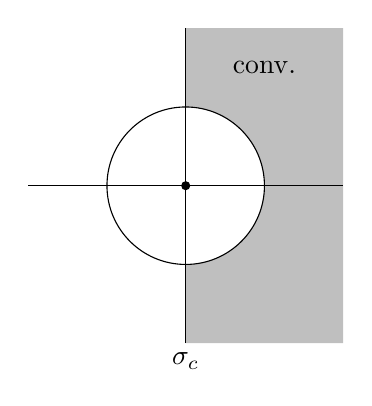
\begin{tikzpicture}
\path[fill=lightgray](0,2)--(0,1)arc(90:-90:1)--(0,-2)--(2,-2)--(2,2)--cycle;
\draw(-2,0)--(2,0);
\draw(0,-2)--(0,2);
\draw[fill](0,0)circle(0.05);
\draw(0,0)circle(1);
\node[below]at(0,-2){$\sigma_c$};
\node at(1,1.5){conv.};
\end{tikzpicture} \]
